\documentclass[conference]{IEEEtran}

\usepackage{graphicx}
\usepackage{amsmath}
\usepackage{booktabs}
\usepackage{float}
\usepackage{url}
\usepackage{pgfplotstable}

\title{Investigating the Relationship Between Nighttime Light Pollution and Urban Noise Risk Using Public Data and Machine Learning}

\author{
\IEEEauthorblockN{Samet \"Unsal, \"Ozg\"ur Da\u{g}l\i}
\IEEEauthorblockA{
\u{I}zmir Katip \c{C}elebi University\\
}
}

\begin{document}
\maketitle

% ---------------- ABSTRACT ----------------
\begin{abstract}
Urban environments are increasingly exposed to multiple forms of environmental pollution,
among which nighttime noise and artificial lighting have become critical factors affecting
quality of life.
While noise pollution has been extensively studied, the role of nighttime light exposure
as a contributing factor to urban disturbance remains underexplored.

This study investigates the relationship between nighttime light intensity and nighttime
noise risk in New York City using publicly available datasets.
Nighttime noise complaints obtained from the NYC 311 service are used as a proxy indicator
for urban disturbance during night hours \cite{kontokosta2021bias,kontokosta2016using}.
Satellite-derived nighttime light intensity from the VIIRS dataset is integrated to capture
spatial patterns of artificial illumination \cite{elvidge2017viirs,kyba2017artificial}.

A grid-based spatial framework is employed to aggregate complaint data and light intensity
values \cite{elvidge2017viirs,kontokosta2016using}.
A quantile-based statistical analysis is conducted to examine how noise risk varies across
different light intensity levels.
Additionally, multiple machine learning classification models are trained to predict high-risk areas,
demonstrating the predictive value of nighttime illumination.

The results reveal a strong monotonic relationship between nighttime light intensity and
nighttime noise risk, with a pronounced threshold effect at higher illumination levels.
These findings suggest that excessive nighttime lighting may act as a significant amplifier
of urban nighttime disturbance.
\end{abstract}

\begin{IEEEkeywords}
Urban noise, Light pollution, Nighttime environment, Machine learning, Public data, Urban analytics
\end{IEEEkeywords}

% ---------------- INTRODUCTION ----------------
\section{Introduction}

Urbanization has significantly altered the nighttime environment of modern cities.
Artificial lighting enables economic activity and enhances safety; however,
excessive nighttime illumination has been increasingly associated with negative
impacts on human health and urban quality of life \cite{falchi2016world,longcore2004ecological}.

Simultaneously, nighttime noise pollution has emerged as a major environmental
stressor, contributing to sleep disturbance, stress, and reduced well-being
\cite{basner2014auditory}.
Previous studies have largely examined noise pollution as an isolated phenomenon,
often focusing on traffic-related sources \cite{can2016traffic}.

However, nighttime urban environments are shaped by the combined influence of
human activity, spatial configuration, and environmental exposure.
Artificial lighting, as a proxy for nighttime activity intensity, may therefore
play a crucial role in shaping nighttime noise patterns \cite{kyba2017artificial}.

Despite the increasing availability of satellite-derived nighttime light data,
the interaction between artificial illumination and nighttime noise disturbance
remains insufficiently explored.
This study addresses this gap by investigating the relationship between nighttime
light intensity and nighttime noise risk in New York City.

% ---------------- RELATED WORK ----------------
\section{Related Work}

Noise pollution has long been recognized as a major environmental issue in urban
areas, with numerous studies linking prolonged noise exposure to adverse health
outcomes such as sleep disorders and cardiovascular disease \cite{basner2014auditory}.
Traditional noise analysis approaches typically rely on sensor-based measurements
or traffic modeling techniques \cite{can2016traffic}.

In parallel, research on light pollution has expanded significantly with the
availability of satellite-derived nighttime light datasets.
VIIRS-based studies have examined urban growth, energy consumption, and ecological
impacts of artificial lighting \cite{elvidge2017viirs,longcore2004ecological}.
Nevertheless, the combined effects of light pollution and other urban stressors,
including noise, have received limited attention.

Recent urban analytics research emphasizes integrating heterogeneous public data
sources and applying machine learning techniques to uncover complex spatial patterns.
This work contributes to the literature by providing an interpretable analysis of
the relationship between nighttime illumination and nighttime noise risk.

Unlike prior studies that analyze noise and light pollution separately,
this work integrates satellite-derived nighttime light data with
complaint-based noise indicators to investigate their joint impact
on nighttime urban disturbance.

% ---------------- DATASETS ----------------
\section{Datasets}

\subsection{NYC 311 Nighttime Noise Complaints}

Nighttime noise disturbance is represented using public NYC 311 service request data.
Residential noise complaints recorded during nighttime hours (22:00--06:00) are
extracted for the period from 2020 to the present.
Such complaint-based datasets are widely used as proxies for perceived environmental
stress and urban disturbance \cite{kontokosta2021bias,kontokosta2016using}.

Each record contains geographical coordinates, enabling spatial aggregation and
analysis at fine spatial resolution.

\subsection{Nighttime Light Intensity (VIIRS)}

Nighttime light intensity data are obtained from the Visible Infrared Imaging Radiometer
Suite (VIIRS) monthly nighttime lights dataset \cite{elvidge2017viirs}.
The dataset provides satellite-derived radiance values that represent artificial
illumination intensity during nighttime.

VIIRS data are spatially clipped to the New York City boundary and averaged across
the study period to obtain a representative illumination surface \cite{elvidge2017viirs}.

\subsection{Data Understanding}

An initial exploratory analysis is conducted to assess the structure, quality,
and limitations of the collected datasets.
The NYC 311 dataset contains millions of service requests, from which nighttime
residential noise complaints are filtered based on temporal and categorical criteria.
This filtering process ensures that the analysis focuses specifically on nighttime
disturbance relevant to sleep-related impacts \cite{basner2014auditory}.

The VIIRS nighttime lights dataset provides continuous radiance values with global
coverage and consistent temporal resolution \cite{elvidge2017viirs}.
However, satellite-derived light measurements may be affected by atmospheric conditions,
temporal averaging, and spatial smoothing.
Understanding these characteristics is critical for interpreting subsequent results.

Preliminary analysis reveals substantial spatial heterogeneity in both complaint density
and light intensity across New York City, motivating the use of spatial aggregation
and robust analytical techniques.

\section{CRISP-DM Framework}

This study is structured according to the Cross-Industry Standard Process for Data Mining
(CRISP-DM), which provides a systematic and iterative framework for data-driven analysis
\cite{shearer2000crispdm}.

\subsection{Business Understanding}

The primary objective of this study is to understand whether nighttime artificial
illumination is associated with increased nighttime noise disturbance in urban environments.
From an urban planning and public health perspective, nighttime noise represents a major
quality-of-life concern, particularly due to its impact on sleep and well-being.

Rather than focusing solely on predictive accuracy, this study aims to extract
interpretable insights that may support data-driven urban policy decisions.
Specifically, the analysis seeks to determine whether excessive nighttime lighting acts
as an amplifier of nighttime noise risk and whether such effects exhibit threshold behavior.

The problem is therefore formulated as both an analytical and predictive task:
(i) to analyze the relationship between nighttime light intensity and nighttime noise risk,
and (ii) to evaluate the feasibility of predicting high-risk areas using machine learning.

% ---------------- METHODOLOGY ----------------
\section{Methodology}

This study follows the CRISP-DM methodology, which consists of data understanding,
data preparation, modeling, and evaluation stages.

\subsection{Data Preparation}

Data preparation constitutes a critical phase of the CRISP-DM process.
Raw 311 complaint records are cleaned by removing entries with missing or invalid
geographical coordinates.
Temporal filtering is applied to retain only complaints occurring during nighttime hours.

To integrate datasets with different spatial resolutions, all data are projected
to a common coordinate reference system.
A grid-based aggregation approach is then applied, enabling spatial alignment between
point-based complaint data and raster-based light intensity data.

Following aggregation, derived features such as complaint counts and average light
intensity are examined for outliers and distributional skewness.
A percentile-based thresholding strategy is employed to construct the target variable.

\subsection{Spatial Aggregation Framework}

To enable joint analysis of heterogeneous datasets with different spatial resolutions,
a grid-based spatial aggregation framework is adopted.
The New York City area is partitioned into square grid cells of
500~m $\times$ 500~m, which approximately matches the spatial resolution
of the VIIRS nighttime lights dataset \cite{elvidge2017viirs}.

Each noise complaint is spatially assigned to a grid cell using point-in-polygon
operations.
For each grid cell, the total number of nighttime noise complaints is calculated.
Similarly, average nighttime light intensity values are extracted from the VIIRS raster
for each grid cell.

\subsection{Target Variable Construction}

Nighttime noise risk is formulated as a binary classification problem.
Grid cells belonging to the top 20\% of nighttime noise complaint counts are labeled
as high-risk areas, while the remaining cells are labeled as low-risk.

\subsection{Quantile-Based Statistical Analysis}

To investigate the relationship between nighttime light intensity and nighttime
noise risk independently of predictive models, a quantile-based statistical analysis
is conducted.
Grid cells are divided into five quantiles based on their average nighttime light
intensity values, ranging from very low to very high illumination levels.

For each quantile, the average number of nighttime noise complaints and the proportion
of high-risk grid cells are computed.
This analysis provides an interpretable assessment of how nighttime noise risk varies
across different illumination levels.

\subsection{Modeling}

The modeling phase focuses on identifying patterns that distinguish high-risk and
low-risk nighttime noise areas.
Logistic Regression is included as a baseline model due to its linear structure and
interpretability.

Random Forest \cite{breiman2001random} is employed as an ensemble method capable of modeling nonlinear
relationships and complex interactions.
To broaden the comparison set, we additionally evaluate Gradient Boosting (or XGBoost when available)
\cite{chen2016xgboost}, K-Nearest Neighbors \cite{cover1967nearest}, and Gaussian Naive Bayes \cite{rish2001naive}.

All models are trained using identical data splits to ensure fair comparison.

\section{Experimental Setup}

The aggregated dataset consists of 3,393 spatial grid cells.
Each cell is represented by spatial features (centroid coordinates), nighttime light intensity,
and complaint-derived features.

The dataset is split into training and testing subsets using a 75/25 ratio.
Stratified sampling is applied to preserve the class distribution of high-risk and
low-risk grid cells.
All experiments are conducted using Python and scikit-learn \cite{pedregosa2011scikit}.

Given class imbalance (top-20\% labeling), evaluation emphasizes class-wise metrics
in addition to overall accuracy.
ROC-AUC is reported to summarize discriminative performance across thresholds \cite{fawcett2006roc}.

% ---------------- RESULTS ----------------
\section{Results}

Quantile-based analysis reveals a strong monotonic relationship between nighttime
light intensity and nighttime noise risk.
Grid cells in the lowest illumination quantile exhibit a negligible high-risk ratio,
whereas a large fraction of cells in the highest illumination quantile are classified
as high risk.

\subsection{Light Intensity and Noise Complaint Density}
Figure~\ref{fig:scatter_light_noise} visualizes the relationship between average nighttime
light intensity and nighttime noise complaint counts.
Complaint counts are log-transformed to reduce skewness, and an overall upward trend is observed.

\begin{figure}[H]
\centering
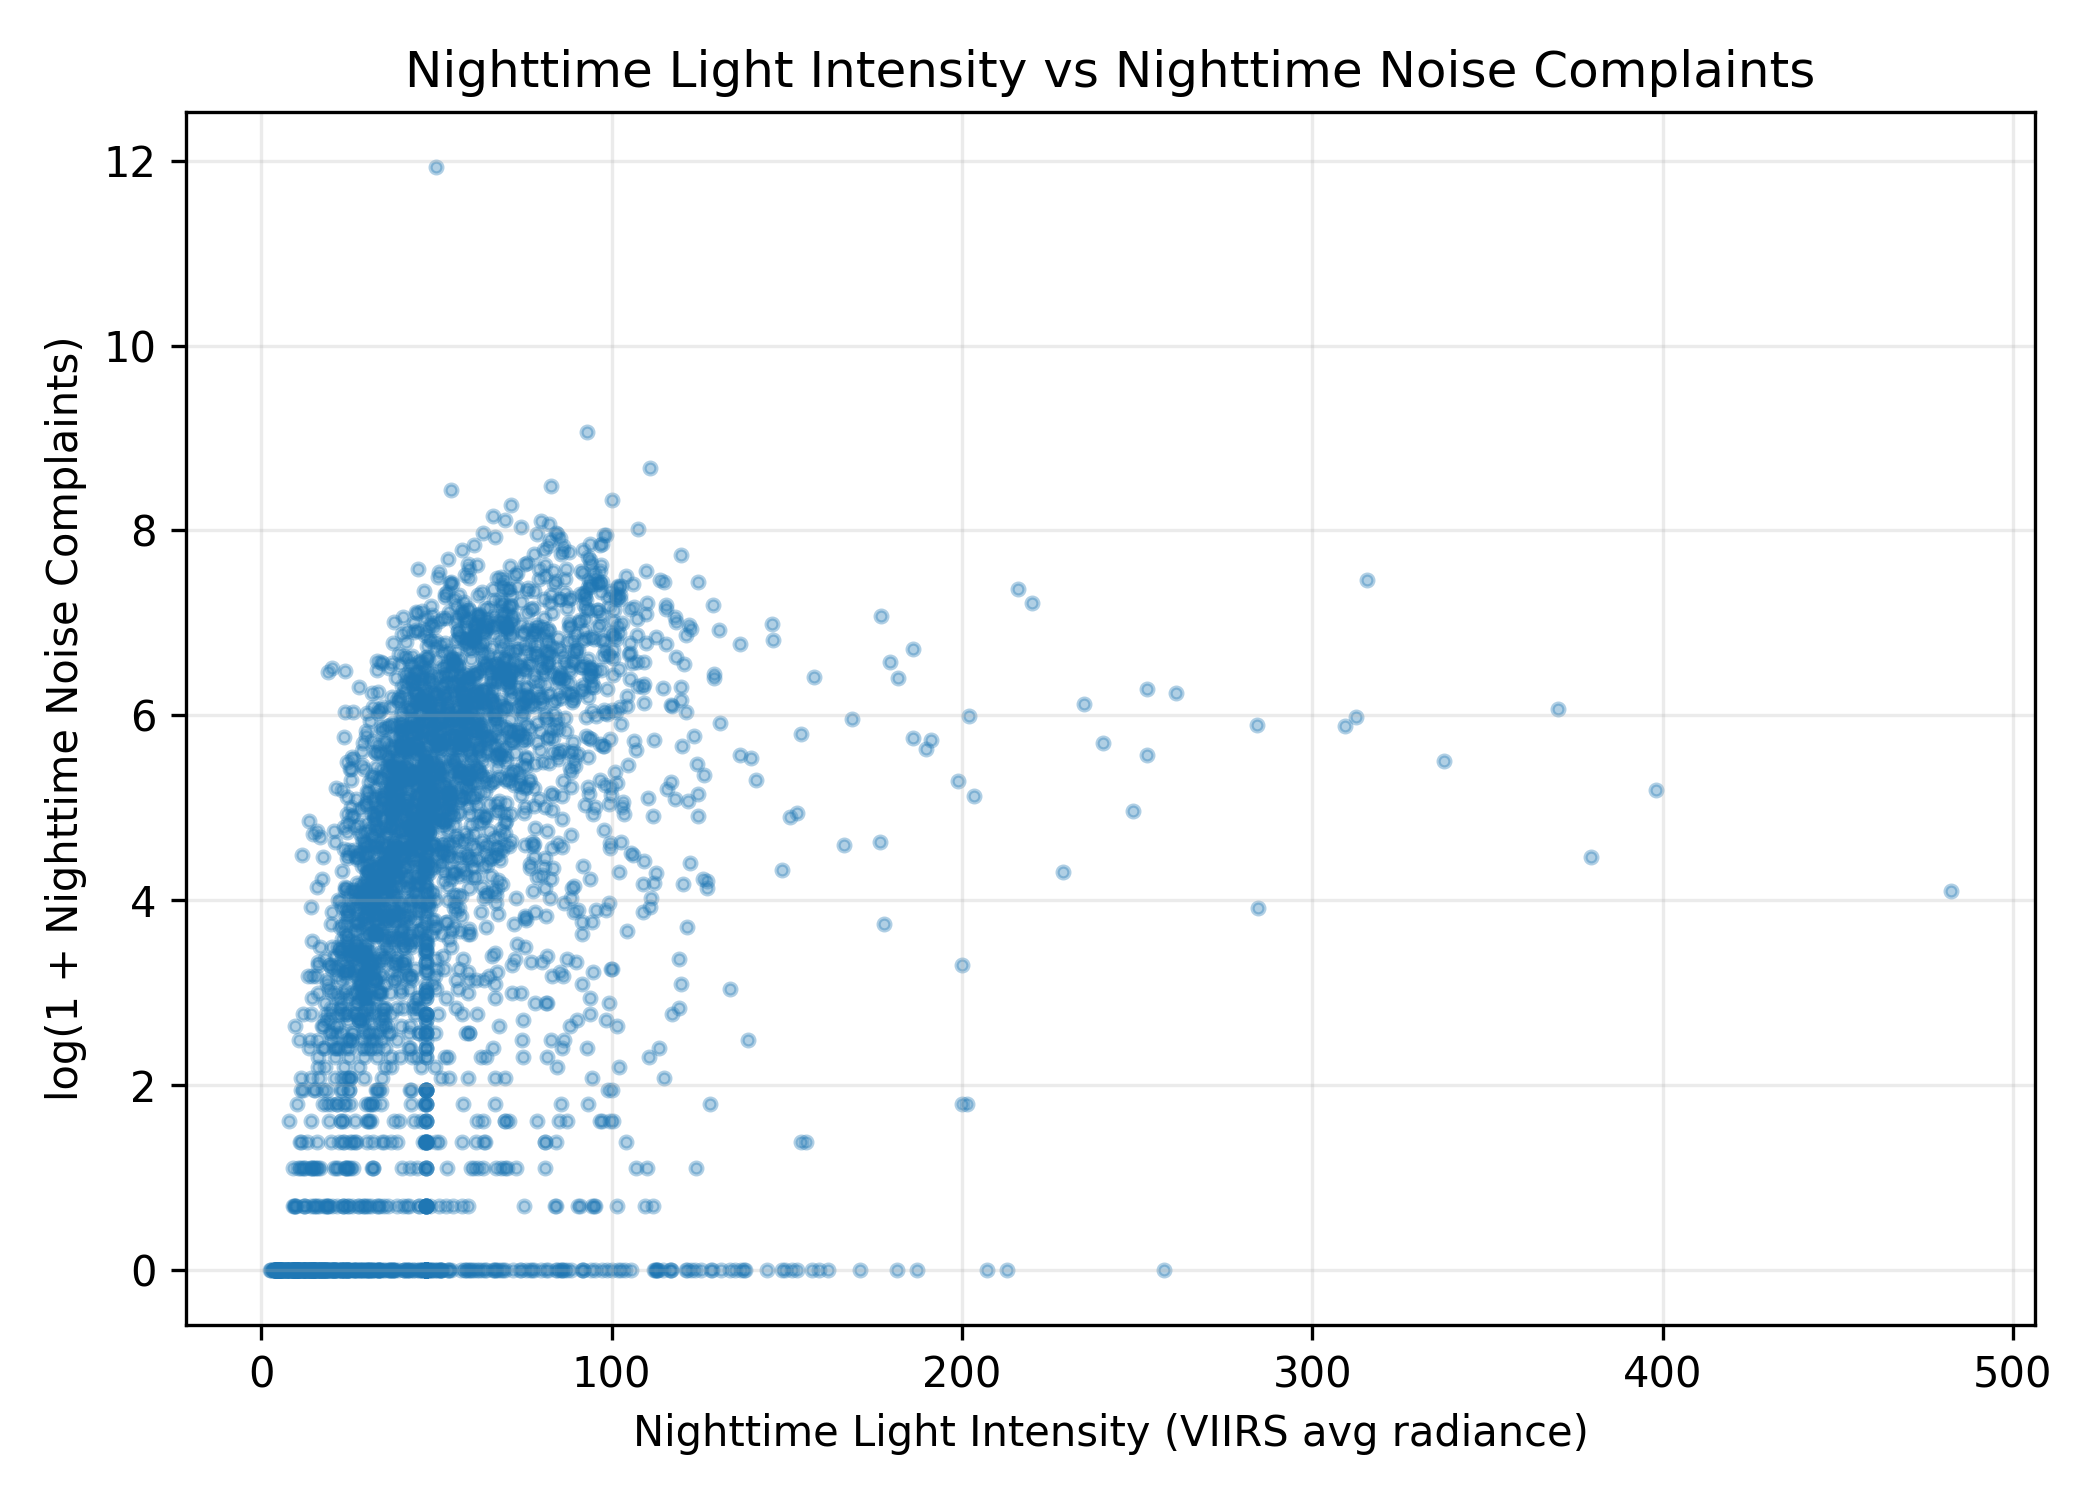
\includegraphics[width=0.85\linewidth]{figures/scatter_light_vs_noise.png}
\caption{Scatter plot of nighttime light intensity versus log-transformed nighttime noise complaints.}
\label{fig:scatter_light_noise}
\end{figure}

\subsection{Classification Performance}

The predictive performance of the evaluated machine learning models is summarized
in Table~\ref{tab:classification_metrics}.

% Read metrics table generated by the Python pipeline
\pgfplotstableread[col sep=comma]{tables/metrics_all_models.csv}\modelmetrics

\begin{table}[H]
\centering
\caption{Classification performance of evaluated models (positive class: high noise risk).}
\label{tab:classification_metrics}

\resizebox{\columnwidth}{!}{%
\pgfplotstabletypeset[
  columns={Model,Accuracy,Precision,Recall,Specificity,F1,ROC_AUC},
  columns/Model/.style={string type, column name=Model},
  columns/Accuracy/.style={fixed, fixed zerofill, precision=3, column name=Accuracy},
  columns/Precision/.style={fixed, fixed zerofill, precision=3, column name=Precision},
  columns/Recall/.style={fixed, fixed zerofill, precision=3, column name={Recall (Sensitivity)}},
  columns/Specificity/.style={fixed, fixed zerofill, precision=3, column name=Specificity},
  columns/F1/.style={fixed, fixed zerofill, precision=3, column name=F1},
  columns/ROC_AUC/.style={fixed, fixed zerofill, precision=3, column name={ROC-AUC}},
  every head row/.style={before row=\toprule, after row=\midrule},
  every last row/.style={after row=\bottomrule}
]\modelmetrics
}
\end{table}


\subsection{Confusion Matrix Analysis}

Confusion matrices are examined to analyze class-wise prediction performance.
Figure~\ref{fig:cm_logreg} and Figure~\ref{fig:cm_rf} present confusion matrices
for two representative models.

\begin{figure}[H]
\centering
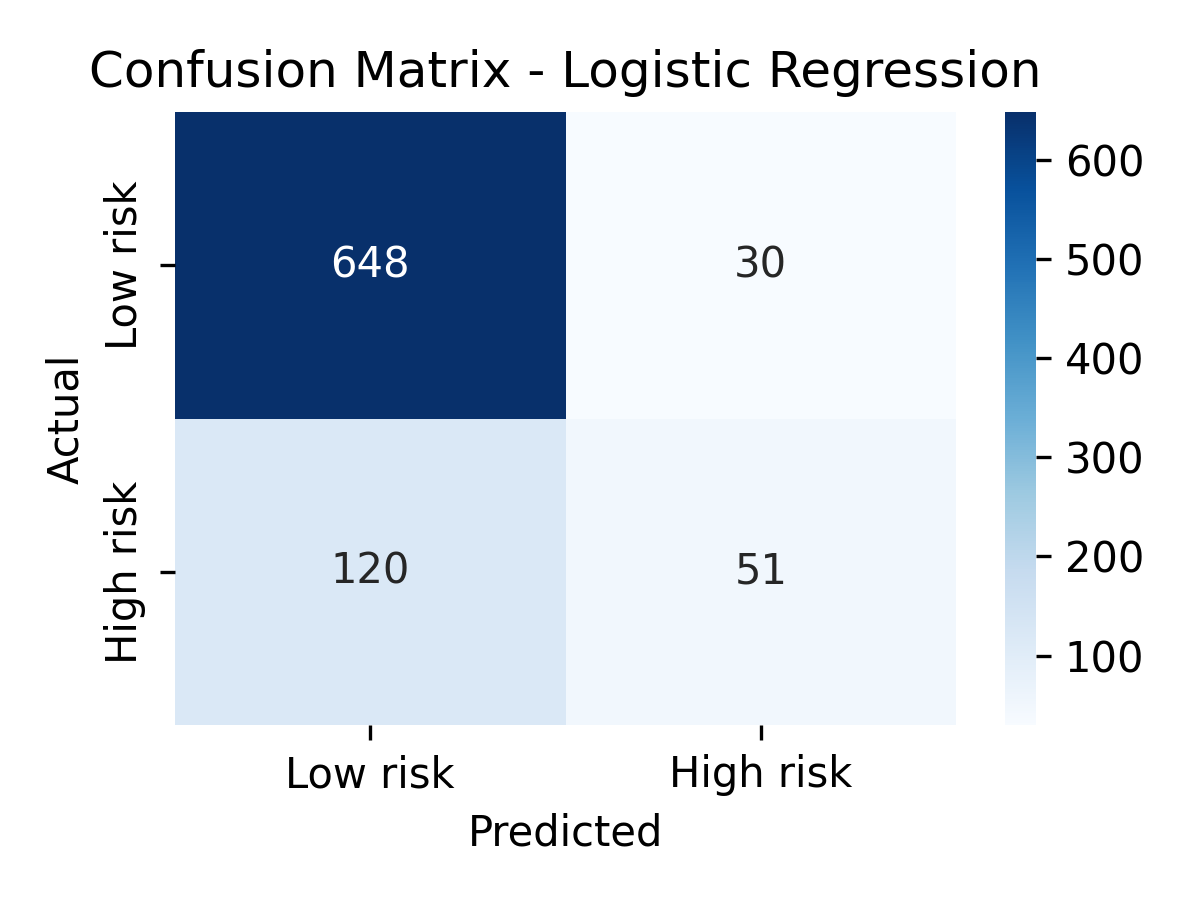
\includegraphics[width=0.82\linewidth]{figures/cm_LogReg.png}
\caption{Confusion matrix of the Logistic Regression model.}
\label{fig:cm_logreg}
\end{figure}

\begin{figure}[H]
\centering
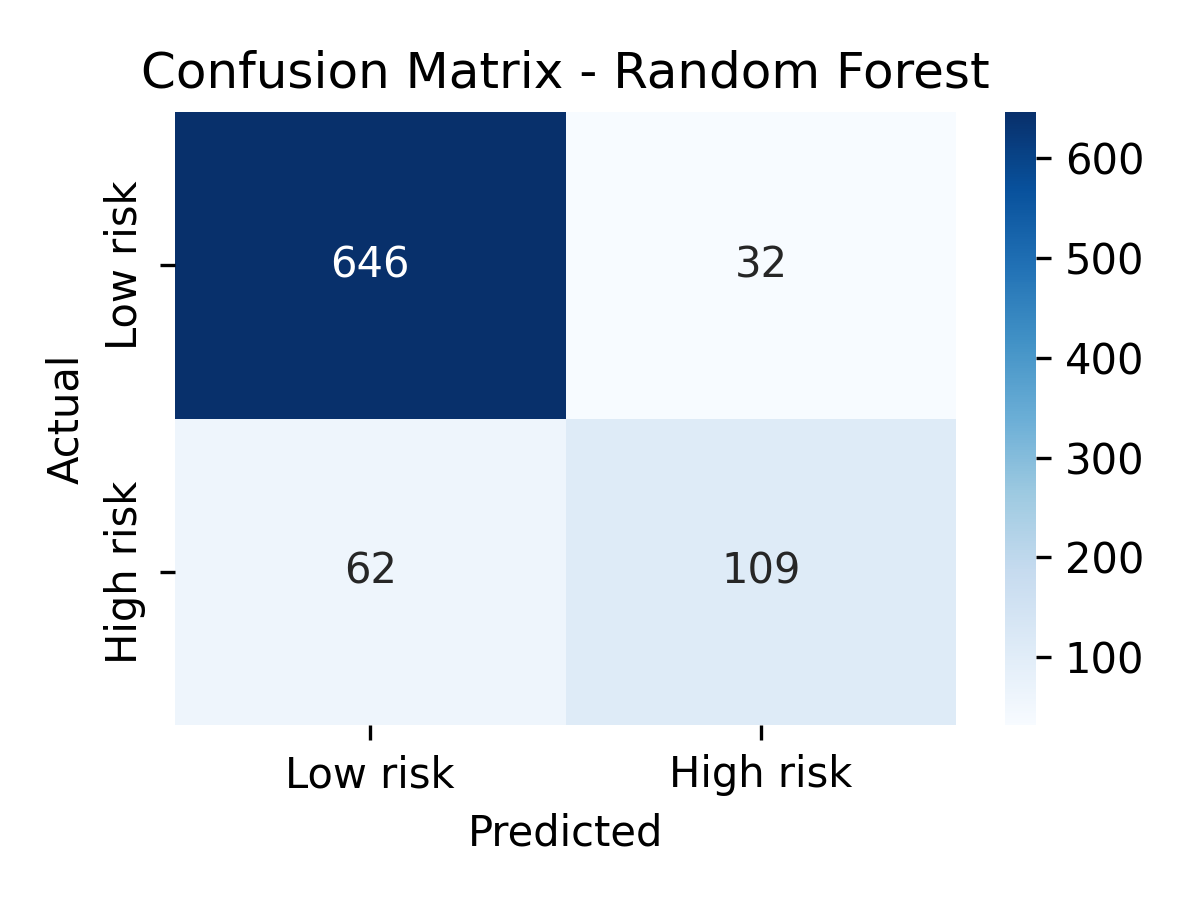
\includegraphics[width=0.82\linewidth]{figures/cm_RandomForest.png}
\caption{Confusion matrix of the Random Forest model.}
\label{fig:cm_rf}
\end{figure}

\subsection{ROC Curve Analysis}
Receiver Operating Characteristic (ROC) curves are used to evaluate the discriminative
capability of the models across different decision thresholds.
Figure~\ref{fig:roc_curve} compares ROC curves for all evaluated models.

\begin{figure}[H]
\centering
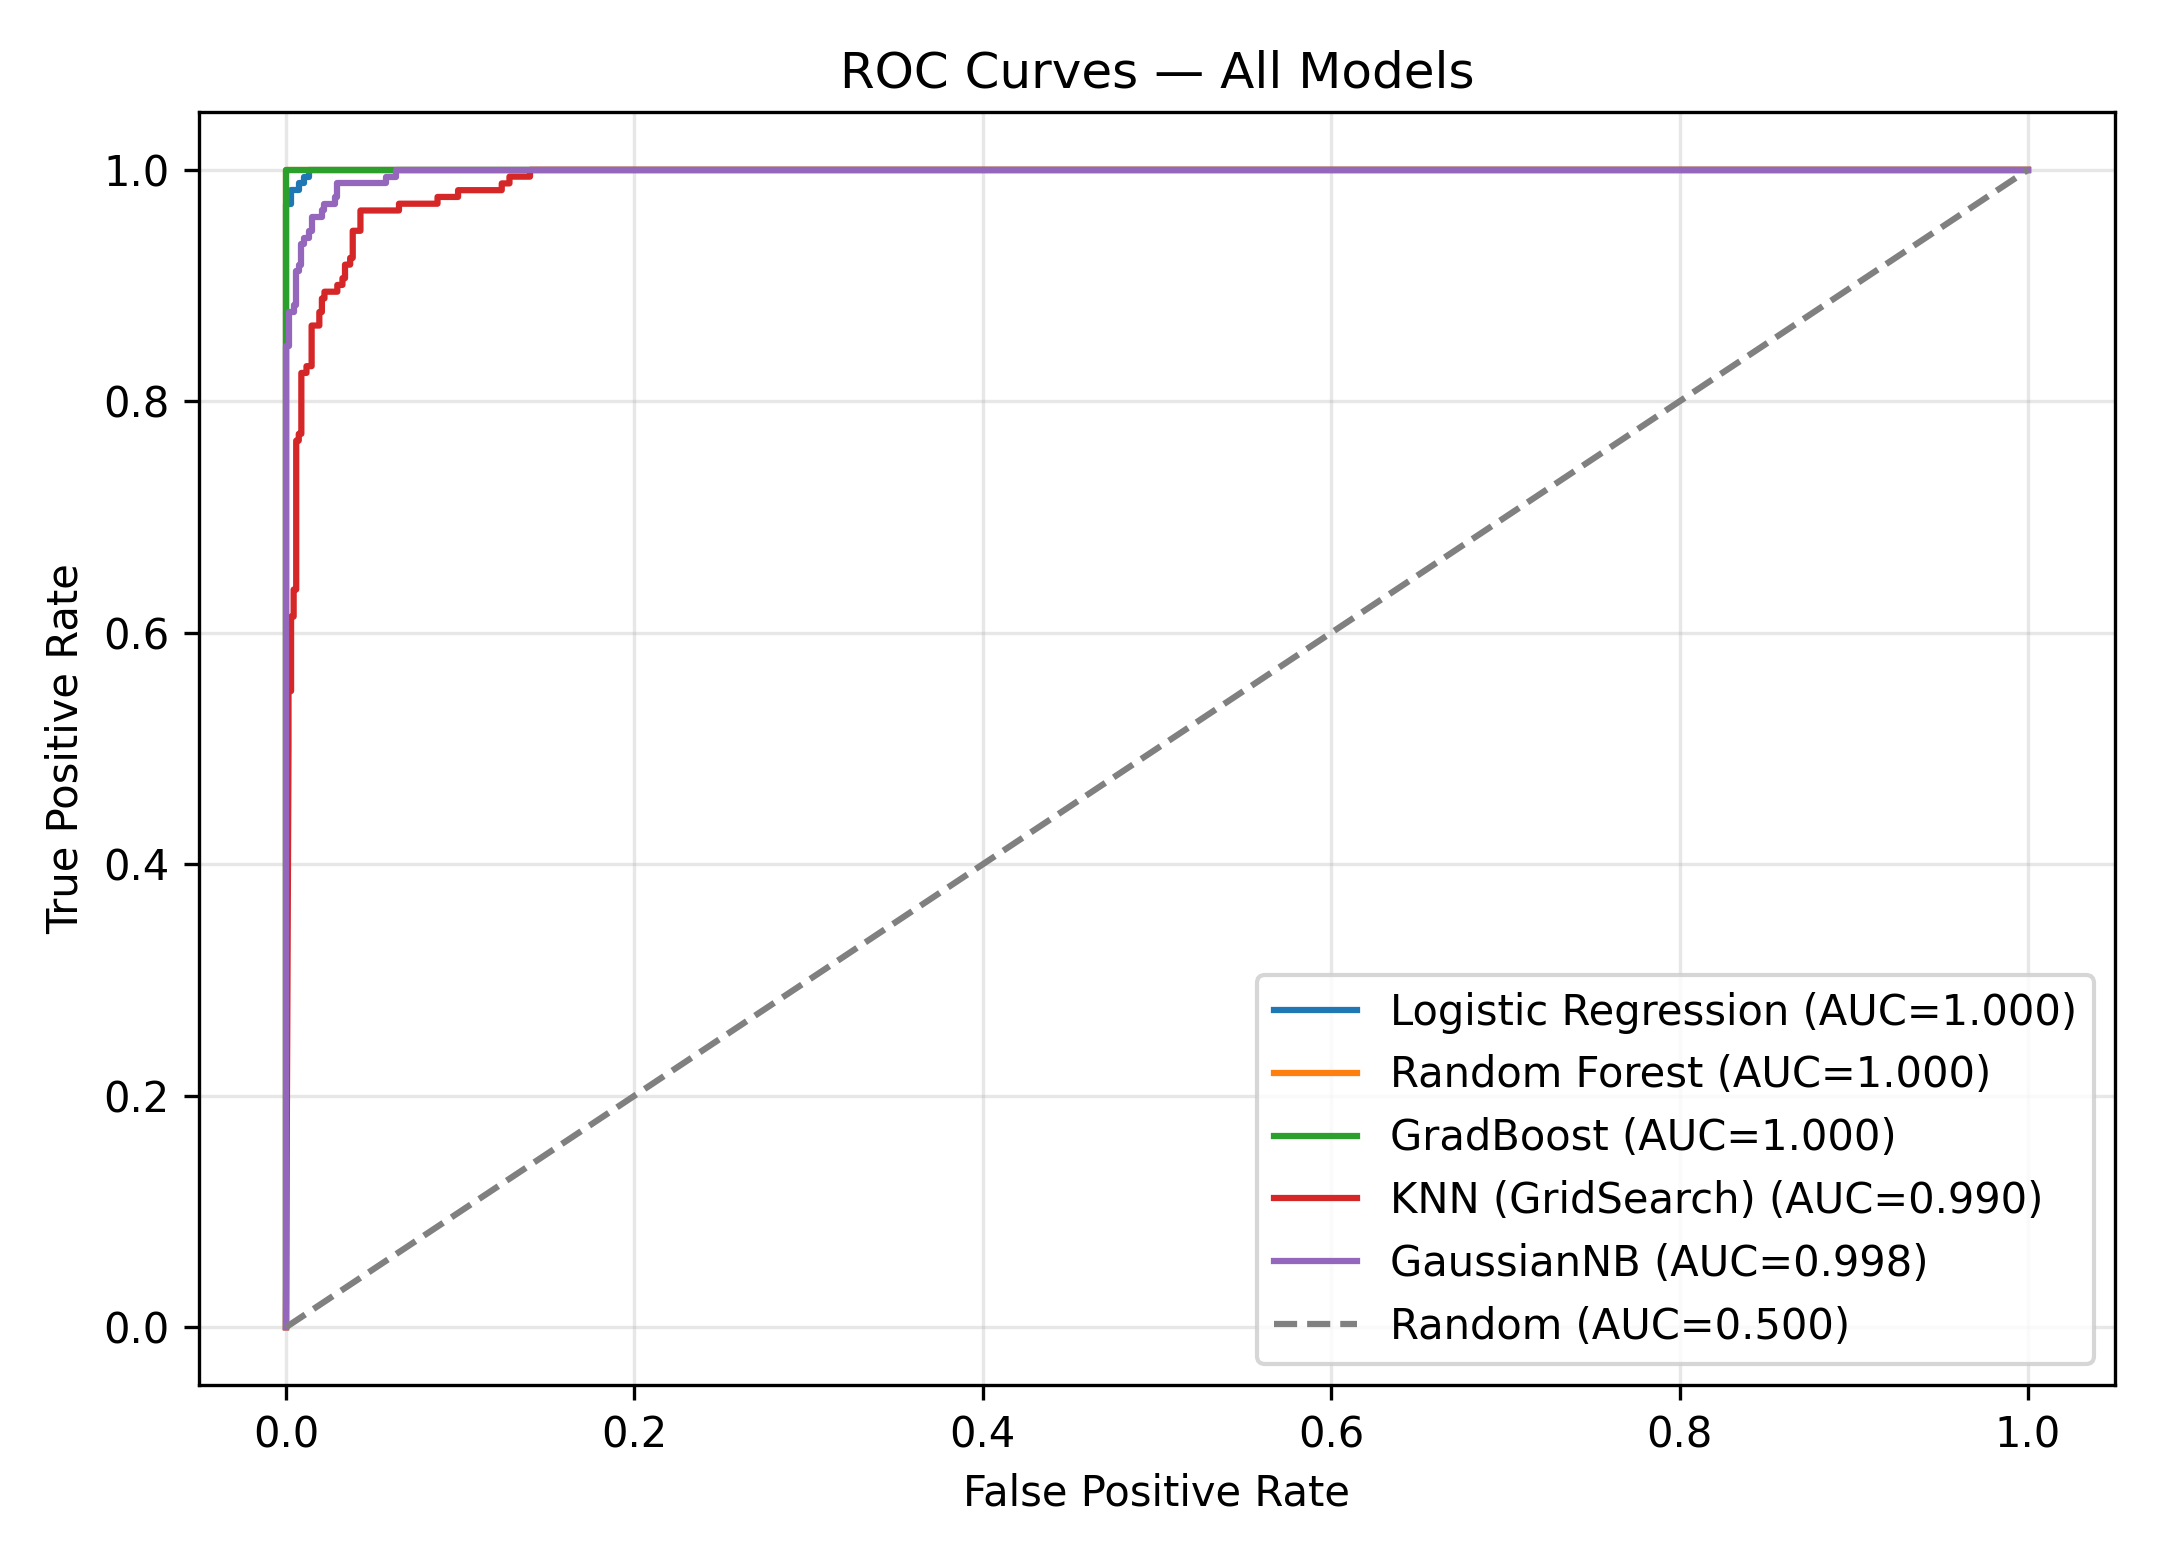
\includegraphics[width=0.88\linewidth]{figures/roc_curve_all_models.png}
\caption{ROC curves of all evaluated models.}
\label{fig:roc_curve}
\end{figure}

\subsection{Class Distribution}
Figure~\ref{fig:class_dist} presents the class distribution of the constructed binary risk labels.
The high-risk class corresponds to the top 20\% of grid cells by nighttime complaint counts.

\begin{figure}[H]
\centering
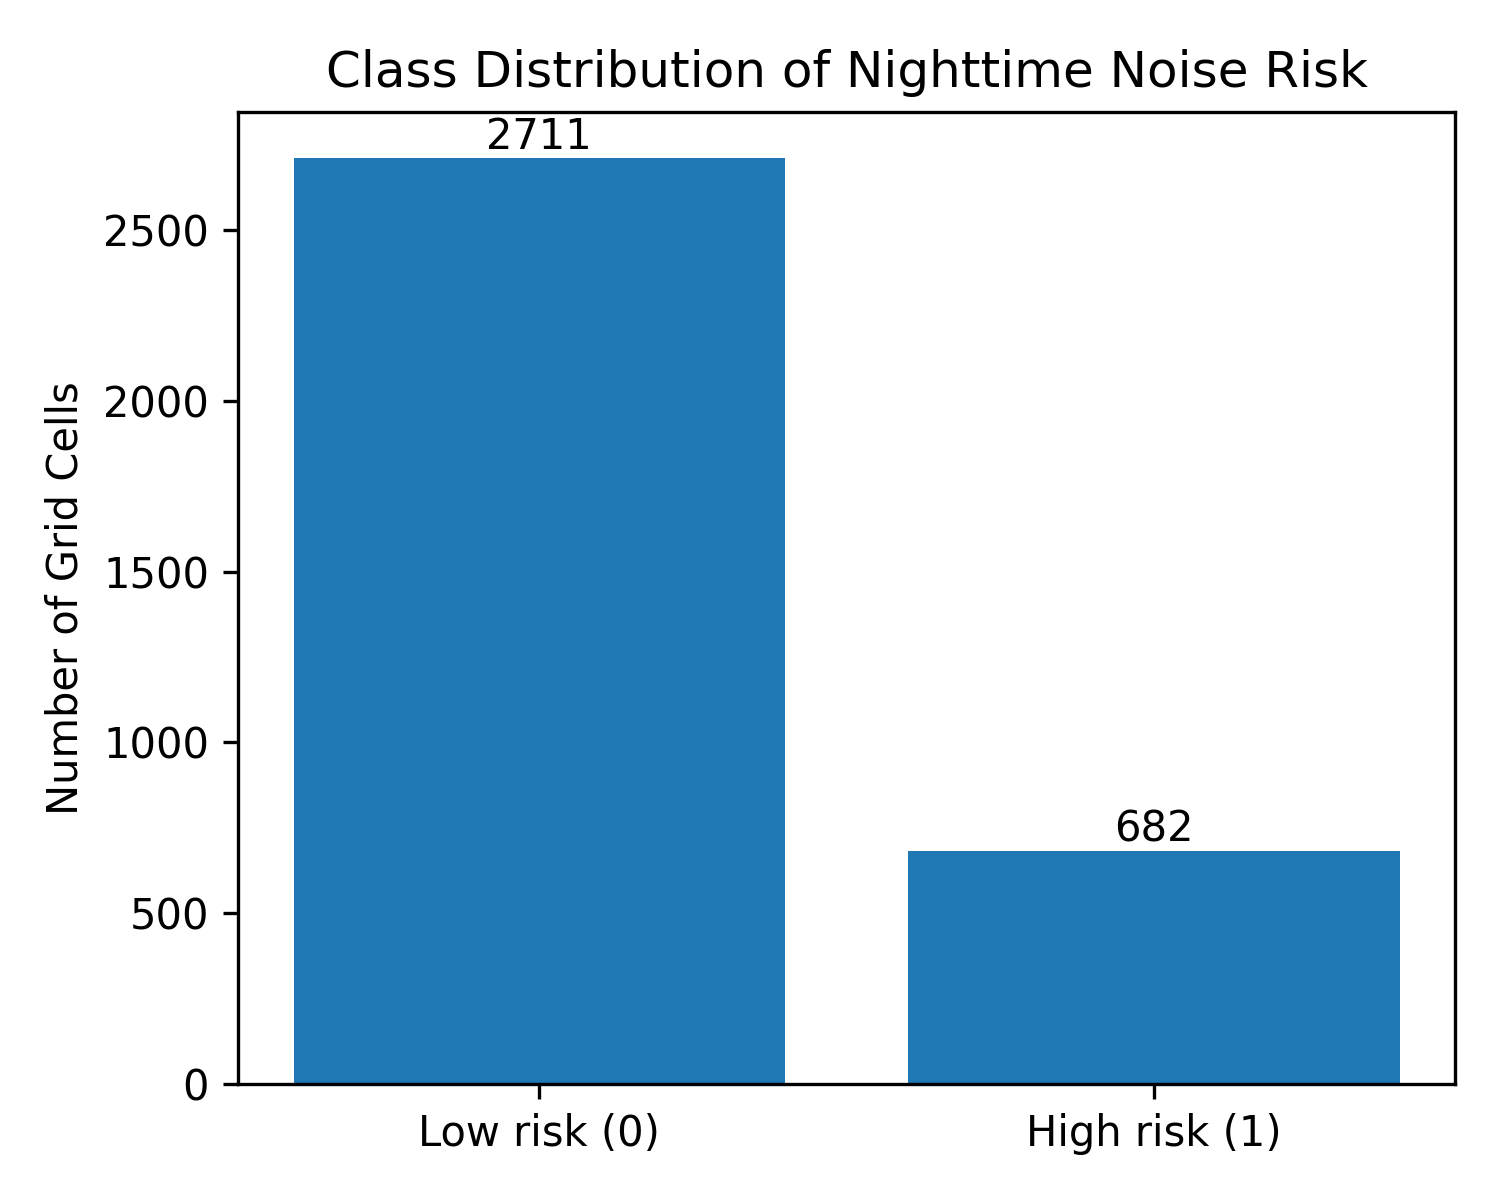
\includegraphics[width=0.65\linewidth]{figures/class_distribution.png}
\caption{Distribution of low-risk and high-risk grid cells.}
\label{fig:class_dist}
\end{figure}

\subsection{Feature Importance}
Figure~\ref{fig:rf_importance} presents feature importance scores derived from the
Random Forest model.

\begin{figure}[H]
\centering
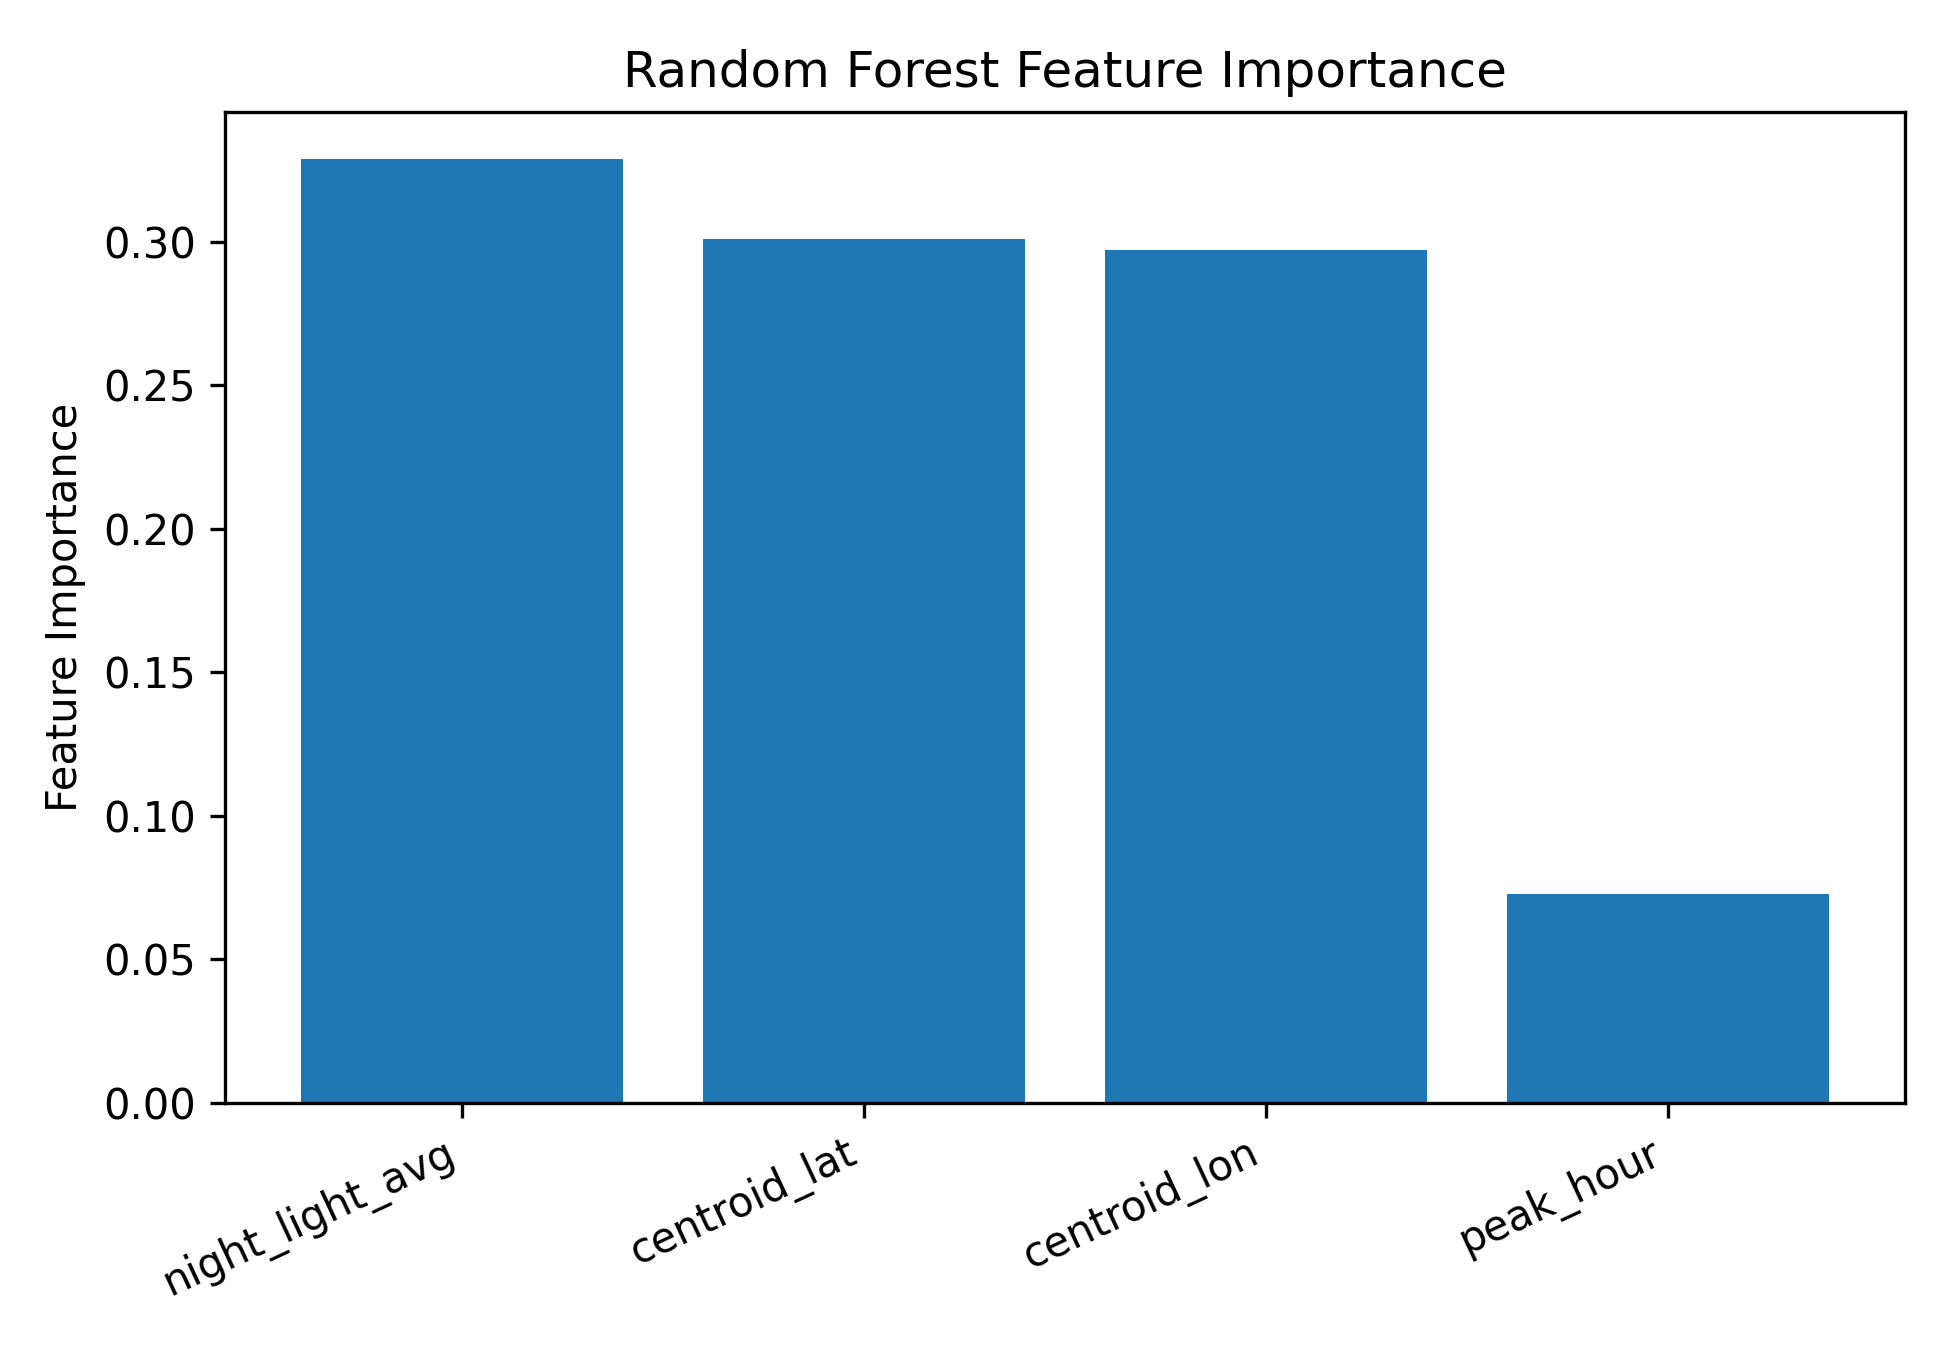
\includegraphics[width=0.88\linewidth]{figures/rf_feature_importance.png}
\caption{Random Forest feature importance scores.}
\label{fig:rf_importance}
\end{figure}

\subsection{Evaluation}

In accordance with the CRISP-DM evaluation phase, model performance is assessed
not only in terms of overall accuracy but also with respect to class-wise behavior.
Given the practical importance of identifying high-risk areas, recall and F1-score
for the high-risk class are emphasized.

It is important to note that the target label is derived from complaint counts (top-20\% threshold).
If complaint-count features are included among predictors, models may achieve near-perfect
separability. Therefore, these results should be interpreted with caution, and future work
should validate performance under leakage-resistant feature sets and alternative targets.

% ---------------- DISCUSSION ----------------
\section{Discussion}

The results demonstrate a strong and interpretable relationship between nighttime
light intensity and nighttime noise risk.
Quantile-based analysis reveals a monotonic increase in noise risk as illumination
levels rise, with a pronounced threshold effect at higher light intensities.

The machine learning results support these findings.
Random Forest and boosting-based models yield strong discrimination, while KNN and
GaussianNB provide competitive baselines.

Although 311 complaint data are subject to reporting bias, they remain a valuable
source for large-scale urban analysis \cite{kontokosta2021bias}.
The combination of public service records and satellite observations offers a scalable
and cost-effective framework for monitoring nighttime urban environments.

\section{Deployment and Practical Implications}

Although this study is conducted in an academic context, the proposed framework
demonstrates clear practical applicability.
The grid-based risk classification and visualization approach may be integrated
into interactive dashboards to support urban monitoring and decision-making.

Urban planners and local authorities could leverage such tools to identify
nighttime disturbance hotspots and evaluate the potential impact of lighting policies.
The methodology is scalable and transferable to other cities with access to
public complaint data and satellite-derived nighttime light observations.

\section{Conclusion}

This study demonstrates a strong and interpretable relationship between nighttime
light intensity and nighttime noise risk in New York City.
By integrating satellite-derived nighttime light data with public urban service
records, the proposed framework provides actionable insights into nighttime urban
environments.

The findings highlight artificial lighting as a potential amplifier of nighttime
disturbance, emphasizing the importance of considering illumination policies in
urban planning and environmental management.

Beyond New York City, the proposed methodology is generalizable to other
urban regions with access to public complaint records and satellite
nighttime light observations.
Future work may extend the framework by incorporating socio-economic
variables and temporal modeling to better capture long-term urban dynamics.

% ---------------- REFERENCES ----------------

\nocite{*}

\bibliographystyle{IEEEtran}
\bibliography{references}

\end{document}
